\documentclass{standalone}
\usepackage{tikz}
\usepackage{times}
\usepackage{amsmath}
\usepackage{txfonts}
\usepackage[utf8]{inputenc}
\usetikzlibrary{backgrounds}

\begin{document}
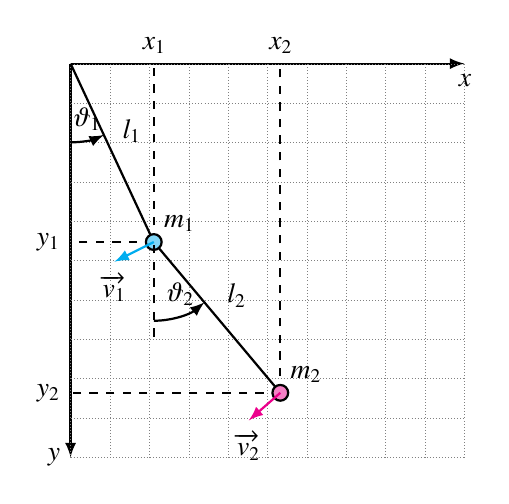
\begin{tikzpicture}[>=latex,thick]

    % Verschiebung des Pendelursprungs nach oben
    \def\pendulumorigin{0,0}

    % Koordinatensystem
    \draw[->] (\pendulumorigin) -- ++(5,0) node[below] {$x$};
    \draw[->] (\pendulumorigin) -- ++(0,-5) node[left] {$y$};

    % Zeichnung des karierten Gitters im Hintergrund
    \def\rows{0} % Anzahl der Zeilen
    \def\cols{5} % Anzahl der Spalten
    \def\spacing{0.5} % Abstand zwischen den Linien

    \draw[step=\spacing,gray,densely dotted, ultra thin] (0,-5) 
    grid (\cols,\rows);

    % Parameter
    \def\lone{2.5} % Länge der ersten Stange
    \def\ltwo{2.5} % Länge der zweiten Stange
    \def\thetaone{25} % Winkel theta1
    \def\thetatwo{40} % Winkel theta2
    \def\mone{0.7} % Masse m1
    \def\mtwo{0.7} % Masse m2

    % Berechnung der Positionen der Massen
    \pgfmathsetmacro{\moneposx}{\lone*sin(\thetaone)}
    \pgfmathsetmacro{\moneposy}{-\lone*cos(\thetaone)}
    \coordinate (m1) at (\moneposx,\moneposy);
    \pgfmathsetmacro{\mtwoposx}{\moneposx + \ltwo*sin(\thetatwo)}
    \pgfmathsetmacro{\mtwoposy}{\moneposy - \ltwo*cos(\thetatwo)}
    \coordinate (m2) at (\mtwoposx,\mtwoposy);

    % Position der Massen im Koordinatensystem
    \draw[dashed] (m1) -- (0,\moneposy) node[left] {\(y_1\)};
    \draw[dashed] (m2) -- (0,\mtwoposy) node[left] {\(y_2\)};
    \draw[dashed] (m1) -- (\moneposx,0) node[above] {\(x_1\)};
    \draw[dashed] (m2) -- (\mtwoposx,0) node[above] {\(x_2\)};

    % Zeichnung der Stangen
    \draw (\pendulumorigin) -- (m1) node[midway,above right] {\(l_1\)};
    \draw (m1) -- (m2) node[midway,above right] {\(l_2\)};

    % Zeichnung der Pendelmassen als Kugeln
    \filldraw[fill=cyan!50] (m1) circle (0.1) node[above right] {\(m_1\)};
    \filldraw[fill=magenta!50] (m2) circle (0.1) node[above right] {\(m_2\)};

    % Zeichnung der Winkel
    \draw[->] ++(0,-1) arc (-90:\thetaone-90:1) node[midway,above] 
    {\(\vartheta_1\)};
    \draw[->] ++(\moneposx,\moneposy-1) arc (-90:\thetatwo-90:1) 
    node[midway,above] {\(\vartheta_2\)};
    \draw[dashed] (\moneposx,\moneposy-1.2) -- (m1);

    % Vektorlänge und Winkel
    \draw[->,-latex,thick,draw=cyan] (\moneposx, \moneposy) -- (\moneposx-0.5, \moneposy-0.25)
    node[below] {\(\overrightarrow{v_1}\)};
    \draw[->,-latex,thick,draw=magenta] (\mtwoposx, \mtwoposy) -- (\mtwoposx-0.4, \mtwoposy-0.35)
    node[below] {\(\overrightarrow{v_2}\)};

\end{tikzpicture}
\end{document}
